\documentclass[10pt,a4paper]{article}
\usepackage[utf8]{inputenc}
\usepackage[english,russian]{babel}
\usepackage{cmap}
\usepackage[OT1]{fontenc}
\usepackage{amsmath}
\usepackage{amsfonts}
\usepackage{amssymb}
\usepackage{graphicx}
\usepackage{float}
\usepackage{wrapfig}
\usepackage{caption}
\DeclareCaptionLabelSeparator{dot}{. }
\captionsetup{justification=centering,labelsep=dot}
\graphicspath{{pictures/}}
\DeclareGraphicsExtensions{.pdf,.png,.jpg,.eps}
\begin{document}


\part{Картографирование}

\textbf{9	Картографирование с помощью сеток занятости}\\

\textbf{9.1	Введение}\\

В предыдущих двух главах обсуждалось применение вероятностных методов в задачах восприятия с низкой размерностью, то есть определение положения робота. При этом подразумевалось, что роботу уже дана предварительно созданная карта. Такое допущение справедливо для очень малого количества реальных сценариев, в которых карты априори доступны или же могут быть созданы вручную. В некоторых областях применения такой роскоши, как предварительно доступная карта, не бывает. Удивительно, но для большинства зданий недоступны планы помещений, созданные их архитекторами. И даже если планы имеются в наличии (и они точны), на них не обозначены мебель и прочие элементы, которые, с точки зрения робота, определяют конфигурацию среды в той же степени, что окна и двери. Возможность построить карту «с нуля» может сильно уменьшить необходимые для установки мобильного робота усилия и позволит адаптироваться к изменениям среды без участия человека. Фактически, картографирование является одной из базовых возможностей по-настоящему автономных роботов.

Создание карт с помощью мобильных роботов является сложной задачей по целому ряду причин:\\

•	Гипотетическое пространство всех возможных карт невероятно огромно. Поскольку карты определены в непрерывном пространстве, пространство всех карт имеет бесконечную размерность. Даже дискретные приближения, используемые в этой главе, такие, как аппроксимация по сетке, могут быть описаны $10^{5}$ или более переменными. Один только размер такого пространства высокой размерности затрудняет вычисление полных апостериорных распределений для карт. Поэтому подход байесовской фильтрации, который хорошо работал для локализации, непригоден для задачи изучения карт, по крайней мере, в его наивной интерпретации, которая обсуждалась до этого момента.\\

•	Изучение карт представляет собой проблему «курицы и яйца» поэтому часто именуется одновременной локализацией и картографированием (simultaneous localization and mapping - SLAM) или конкурентной проблемой локализации и картографирования (concurrent mapping and localization problem). Во-первых, имеется проблема локализации. Когда робот перемещается в среде, он накапливает ошибки в одометрии, что постепенно увеличивает степень неопределенности относительно его местонахождения. Как было показано в предыдущей главе, существуют методы определения положения робота при условии наличия карты. Во-вторых, имеется проблема картографирования. Создание карты, когда положение робота известно, относительно простая задача. Это утверждение будет подтверждено доказательствами в этой и последующих главах. При отсутствии как изначально заданной карты, так и точных данных о положении робота, необходимо выполнять обе задачи: составлять карту и выполнить локализацию робота относительно этой карты.\\

Конечно, не все проблемы картографирования одинаково трудны. Сложность проблемы картографирования является результатом целого набора факторов, самые важные из которых следующие:\\

•	\textbf{Размер.} Чем больше размер среды относительно расстояния восприятия робота, тем сложнее задача построения карты.\\

•	\textbf{Шумы восприятия и действий.} Если бы датчики и актуаторы робота были идеальны, картографирование превратилось бы в очень простую задачу. Чем выше зашумление, тем сложнее задача.\\

•	\textbf{Двойственность восприятия.} Чем более схожи между собой различные места, тем более сложно установить соответствие между различными местоположениями, через которые в разные моменты времени проходит робот.\\

•\textbf{	Циклы.} Циклы в среде особенно сложны для картографирования. Если робот просто перемещается вперёд и назад по коридору, он может последовательно корректировать по возвращении. Циклы заставляют робота возвращаться разными путями, и при замыкании цикла накопленная ошибка одометрии просто огромна!\\

\begin{figure}[H]
	\center{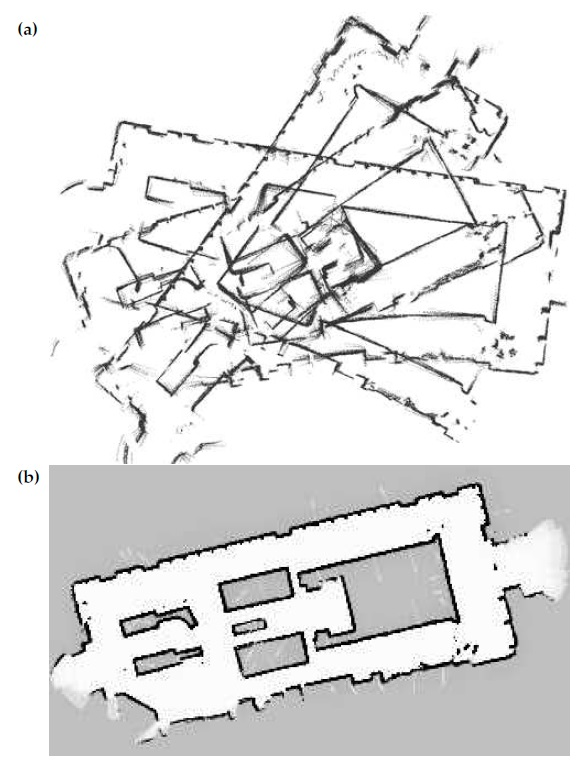
\includegraphics[width=0.8\linewidth]{91orig}}
	\caption{ ( Рис. 9.1 (a) Сырые данные расстояний, положение индексируется одометрией. (b) Карта сетки занятости.)}
	\label{fig:91orig}
\end{figure} 

Чтобы в полной мере оценить сложность задачи картографирования, обратимся к Рис. 9.1. На нем показан набор данных, собранных в большом помещении. Рис. 9.1a был сгенерирован, используя исходные данные одометрии. Каждая чёрная точка на этом рисунке соответствует препятствию, обнаруженному лазерным датчиком расстояния робота. На Рис. 9.1b показан результат применения на этом наборе данных алгоритмов картографии, один из которых описывается в данной главе. Этот пример хорошо иллюстрирует проблему.

В этой главе сначала следует изучить проблему при наличии ограничивающего допущения об известном положении робота. Другими словами, пока отложим в сторону трудности задачи SLAM, и представим, что некий оракул предоставляет точную информацию о пути, пройденном роботом при картографировании.\\
КАРТОГРАФИРОВАНИЕ С ИЗВЕСТНЫМ ПОЛОЖЕНИЕМ\\ 
На Рис. 9.2 представлена задача, также известная как картографирование с известным положением.
Давайте обсудим популярное семейство алгоритмов под общим названием картографирование с помощью сеток занятости, которые решают задачу генерирования непротиворечивых карт из зашумленных и неопределённых данных измерений, при условии, что положение робота известно.  Основная идея карт на основе сеток занятости состоит в представлении карты в виде поля случайных переменных, распределенных по равномерной сетке. Каждая случайная бинарная переменная отображает состояние занятости местоположения, на котором находится. Алгоритмы картографирования на основе сеток занятости реализуют приблизительную апостериорную оценку для этих случайных переменных.

\begin{figure}[H]
	\center{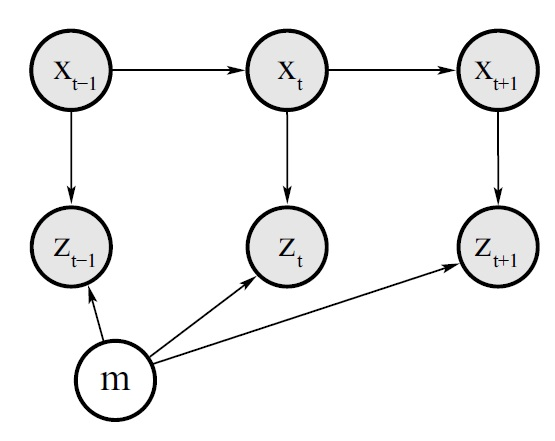
\includegraphics[width=0.6\linewidth]{92orig}}
	\caption{ ( Рис. 9.2 Графическая модель картографирования с известными местоположениями. Переменные, отмеченные цветом (местоположения $x$ и измерения $z$) известны. Целью картографирования является восстановление карты $m$.)}
	\label{fig:92orig}
\end{figure}

Читатель может напомнить о важности метода картографирования, требующего точной информации о положении робота. В конце концов, идеальной одометрии для робота не существует! Основным применением метода сеток занятости является постпроцессинг, поскольку многие из техник SLAM, обсуждаемых в следующих главах, неспособны генерировать карты, подходящие для планирования пути и навигации. Карты сеток занятости часто используются после решения задачи SLAM какими-либо другими методами, принимая результирующие оценочные траектории как данность.\\

\textbf{9.1	Алгоритм картографирования с помощью сеток занятости}\\

Золотым стандартом любого алгоритма картографирования с помощью сеток занятости является вычисление апостериорного распределения по карту на основе имеющихся данных \\

(9.1)
$$p(m|z_{1:t},x_{1:t})$$

Как обычно, $m$ означает карту, $z_{1:t}$  - набор всех измерений до момента времени $t$, а  $x_{1:t}$ траекторию робота, определённую через последовательность всех положений. Сигналы управления $u_{1:t}$ никакой роли в картах сеток занятости не играют, поскольку путь уже известен. Поэтому в этой главе они будут игнорироваться.
 
Для карт сеток занятости используются мелкоячеистые сетки на непрерывных пространствах местоположений. Наиболее популярной областью использования карт сеток занятости являются поэтажные двухмерные карты, которые можно описать в виде плоского среза трехмерной среды. Плоские карты обычно наиболее предпочтительны, если робот действует в горизонтальной среде и датчики дают информацию только об узком её срезе. Методы сеток занятости способны к обобщению до трехмерных представлений, но за счёт существенных вычислительных затрат.

Пусть $m_i$ определяет ячейку сетки с индексом $i$. Карта сеток занятости разбивает пространство на конечное множество ячеек сетки:\\

(9.2)
$$m=\{\textbf{m}_i\}$$

Для каждого $\textbf{m}_i$ имеется бинарное значение занятости, определяющее, свободна ли ячейка. Условимся, что “1” будет обозначать занятые, а “0” - свободные ячейки. Записью $p(\textbf{m}_i = 1)$ или $p(\textbf{m}_i)$ обозначим вероятность занятости данной ячейки сетки.

Проблемой апостериорного распределения в выражении (9.1) является размерность, поскольку количество ячеек сетки на картах наподобие показанной на Рис 9.1 составляет порядка десятков тысяч. Для каждой карты с 10000 ячеек количество вариантов карт, которые можно отобразить с её помощью, составляет $2^{10000}$. Вычисление апостериорной вероятности для каждого варианта карты в таком случае совершенно нецелесообразно.

Стандартный метод сеток занятости разбивает задачу оценки карты на множество отдельных задач оценки\\

(9.3)
$$p(\textbf{m}_i|z_{1:t},x_{1:t})$$

для каждой ячейки сетки $\textbf{m}_i$. Каждая из этих задач оценки представляет собой бинарную задачу статичного состояния. Такая декомпозиция удобна, хотя и имеет ряд ограничений. В частности, она не позволяет отображать зависимости между соседними ячейками, вместо этого апостериорное распределение по всем картам аппроксимируется в виде произведения маргиналов:\\

(9.4)
$$p(m|z_{1:t},x_{1:t})=\prod_i p(\textbf{m}_i|z_{1:t},x_{1:t})$$

Мы вернёмся к этому вопросу чуть ниже в разделе 9.4 при обсуждении более совершенных методов картографирования. Сейчас, для удобства, оставим эту факторизацию.

Из-за факторизации оценка вероятности занятости для каждой ячейки сетки становится бинарной задачей со статическим состоянием. Фильтр для её решения уже обсуждался в разделе 4.2, \textit{это бинарный фильтр Байеса}.   Соответствующий алгоритм приводится в Таблице 4.2 на странице 94 ???.

\begin{table}[H]
\begin{center}
\begin{tabular}{|l|}
\hline
{}\\
1: \textbf{Algorithm occupancy\_grid\_mapping}$(\{l_{t-1,i}\},x_t,z_t):$ \\
2:\hspace{5mm}$\textit{для всех ячеек}\,\,\textbf{m}_i\,\,\textit{do}$\\
3:\hspace{10mm}$\textit{if}\,\,\textbf{m}_i\,\,\textit{в области восприятия}\,\,z_t\,\,\textit{then}$\\
4:\hspace{15mm}$l_{t,i}=l_{t-1,i}+\textbf{inverse\_sensor\_model}(\textbf{m}_i,x_t,z_t)-l_0$\\
5:\hspace{10mm}$\textit{else}$\\
6:\hspace{15mm}$l_{t,i}=l_{t-1,i}$\\
7:\hspace{10mm}$\textit{endif}$\\
8:\hspace{5mm}$\textit{endfor}$\\
9:\hspace{5mm}$\textit{return}\,\,\{l_{t,i}\}$\\
{}\\
\hline
\end{tabular}
\caption{(Таблица 9.1 Алгоритм сетки занятости в версии с бинарным фильтром Байеса из Таблицы 4.2. )}
\end{center}
\end{table}

В алгоритме в Таблице 9.1 этот фильтр используется в задаче картографирования с помощью сеток занятости. Как и в оригинальном фильтре, в предлагаемом алгоритме картографирования с помощью сеток занятости для отображения занятости используется \textit{логарифм шансов}:\\

(9.5)
$$l_{t,i}=\log\frac{p(\textbf{m}_i|z_{1:t},x_{1:t})}{1-p(\textbf{m}_i|z_{1:t}x_{1:t})}$$

Это представление уже знакомо из раздела 4.2. Преимуществом логарифма шансов над представлением в виде вероятности является возможность избежать численной нестабильности для вероятностей вблизи нуля или единицы. Вероятности из отношения логарифма шансов легко восстановить:\\

(9.6)
$$p(\textbf{m}_i|z_{1:t},x_{1:t})=1-\frac{1}{1+\exp\{l_{t,i}\}}$$
 
Алгоритм \textbf{occupancy\_grid\_mapping} в Таблице 9.1 выполняет последовательный проход по всем ячейкам сетки $i$, обновляя те, которые попадают в конус измерения датчика $z_t$. Для таких ячеек значение занятости обновляется с помощью функции \textbf{inverse\_sensor\_model} в строке 4 алгоритма. Для остальных ячеек значение занятости остаётся неизменным, как показано в строке 6. Константа $l_0$ является априорной вероятностью занятости, выраженной в виде отношения логарифма шансов:\\

(9.7)
$$l_0=\log\frac{p(\textbf{m}_i=1)}{p(\textbf{m}_i=0)}=\log\frac{p(\textbf{m}_i)}{1-p(\textbf{m}_i)}$$

\begin{figure}[H]
	\center{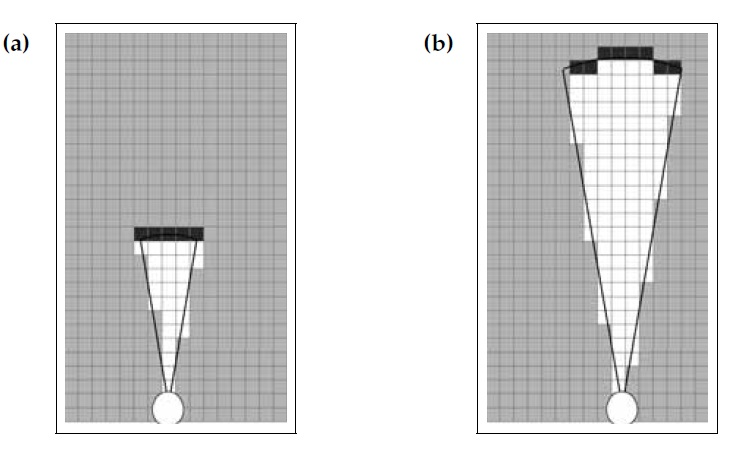
\includegraphics[width=0.8\linewidth]{93orig}}
	\caption{ ( Рис. 9.3 Два примера обратной модели измерения \textbf{inverse\_range\_sensor\_model} для двух различных расстояний измерения. Насыщенность цвета каждой ячейки соответствует правдоподобию её занятости. Модель несколько упрощена, и в современных реализациях вероятности занятости по границам конуса измерения обычно устанавливается ниже.)}
	\label{fig:93orig}
\end{figure}

Функция \textbf{inverse\_sensor\_model} реализует обратную модель измерения $p(\textbf{m}_i | z_t, x_t)$ в виде логарифма шансов:\\

(9.8)
$$\textbf{inverse\_sensor\_model}(\textbf{m}_i,x_t,z_t)=\log\frac{p(\textbf{m}_i|z_t,x_t)}{1-p(\textbf{m}_i|z_t,x_t)}$$

Несколько упрощённый пример такой функции для датчиков расстояния приведён в Таблице 9.2 и показан на Рис. 9.3a и b. Эта модель назначает всем ячейкам в конусе измерений, расстояние до которых близко к данным измерения, значение занятости $l_{occ}$. В Таблице 9.2 указаны ширина области, управляемой параметром $\alpha$, и угол раскрытия луча $\beta$. Обратим внимание на упрощённый характер модели, поскольку в современных реализациях вероятности занятости на границах конуса измерений обычно устанавливается меньше.

Алгоритм \textbf{inverse\_sensor\_model} вычисляет обратную модель определением индекса луча $k$ и расстояния $r$ для центра масс ячейки $\textbf{m}_i$. Это вычисление выполняется в строках с 2 до 5 в Таблице 9.2. Как обычно, допустим, что положение робота задано в виде $x_t = (x\,\,y\,\,\theta)^T$ . В строке 7 возвращается значение априорной вероятности, выраженной в виде логарифма шансов, если ячейка лежит за пределами измеряемого расстояния этого луча датчика или   далее, чем $\alpha/2$ обнаруженного расстояния $z_t^k$. В строке 9 возвращается $l_{occ}>l_0$, если дальность до ячейки более чем на $\pm\alpha/2$ превышает значение обнаруженного расстояния $z_t^k$. Значение $l_{free}<l_0$ возвращается, если расстояние до до ячейки короче измеренного расстояния больше, чем на $\alpha/2$. На левой и центральной панели на Рис. 9.3 показано вычисления основного конуса луча ультразвукового датчика.

\begin{table}[H]
\begin{center}
\begin{tabular}{|l|}
\hline
{}\\
1: \textbf{Algorithm inverse\_range\_sensor\_model}$(\textbf{m}_i,x_t,z_t):$ \\
2:\hspace{5mm}$\textit{Let}\,\,x_i,y_i\,\,\textit{является центром масс}\,\,\textbf{m}_i$\\
3:\hspace{5mm}$r=\sqrt{(x_i-x)^2+(y_i-y)^2}$\\
4:\hspace{5mm}$\phi=\text{atan}2(y_i-y,x_i-x)-\theta$\\
5:\hspace{5mm}$k=\text{argmin}_j|\phi-\theta_{j,sens}|$\\
6:\hspace{5mm}$\textit{if}\,\,r>\text{min}(z_{max},z_t^k+\alpha/2)\,\textit{or}\,|\phi-\theta_{k,sens}|>\beta/2\,\,\textit{then}$\\
7:\hspace{10mm}$\textit{return}\,\,l_0$\\
8:\hspace{5mm}$\textit{if}\,\,z_t^k<z_{max}\,\textit{and}\,|r-z_t^k|<\alpha/2$\\
9:\hspace{10mm}$\textit{return}\,\,l_{\textit{занято}}$\\
10:\hspace{4mm}$\textit{if}\,\,r\leq z_t^k$\\
11:\hspace{9mm}$\textit{return}\,\,l_{\textit{свободно}}$\\
12:\hspace{4mm}$\textit{endif}$\\
{}\\
\hline
\end{tabular}
\caption{(Таблица 9.2 Простая инвертированная модель измерения для робота с ультразвуковыми датчиками расстояния. Здесь $\alpha$ - толщина препятствий, а $\beta$ - ширина луча датчика. Значения $l_{\textit{занято}}$ и $l_{\textit{свободно}}$ в строках 9 и 11 означает степень уверенности, что показания относятся к двум различным случаям.)}
\end{center}
\end{table}

Типичное применение обратной модели датчика для ультразвуковых датчиков показано на Рис. 9.4. Начав с первоначальной картой, робот успешно расширяет ее, учитывая локальные карты, созданные обратной моделью. Карта сетки занятости большего размера, созданная этой моделью для той же среды, показана на Рис. 9.5.

На Рис. 9.6 показан пример карты рядом с планом большого открытого выставочного зала и соотнесение ее с картой сетки занятости, полученной роботом. Карта была сгенерирована, используя собранные за несколько минут данные лазерного датчика расстояния. Насыщенность цвета на карте сетки занятости означает апостериорную вероятность занятости на равномерной сетке. Чем темнее ячейка сети, тем более вероятно, что она занята. Хотя карты занятости изначально вероятностные, они быстро сводятся к двум граничным вероятностям, 1 и 0. При сравнении сгенерированной карты и плана видно, что на карте сетки занятости показаны все основные структурные элементы и препятствия, видимые с высоты лазера. При внимательном изучении читатель может заметить некоторые небольшие несоответствия между планами и настоящей конфигурацией среды.

\begin{figure}[H]
	\center{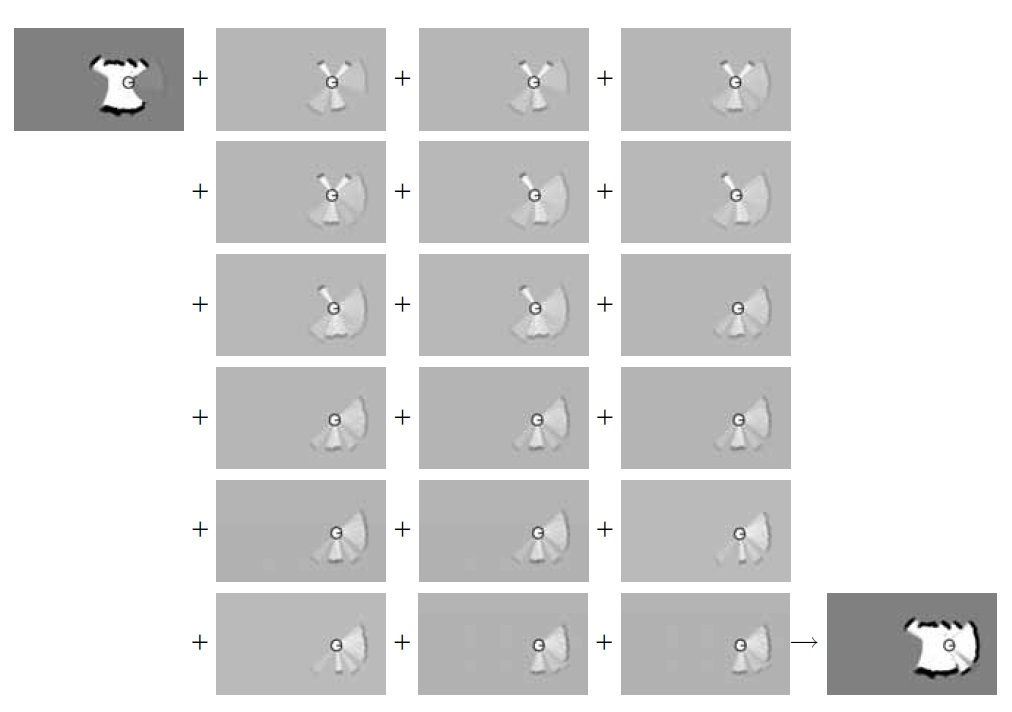
\includegraphics[width=0.9\linewidth]{94orig}}
	\caption{ ( Рис. 9.4 последовательное построение карты сетки занятости, используя данные ультразвукового датчика в среде в виде коридора. В левом верхнем углу показана начальная карта, а в правом нижнем – результирующая карта. В колонках со 2 по 4 показаны локальные карты, построенные или обратной модели датчика. Измерения за пределами радиуса 2,5 м не учитываются. Угол раскрытия каждого конуса измерения составляет 15 градусов. Изображения принадлежат Сириллу Стачнису из Университета Фрайбурга (Cyrill Stachniss, University of Freiburg).)}
	\label{fig:94orig}
\end{figure}

\begin{figure}[H]
	\center{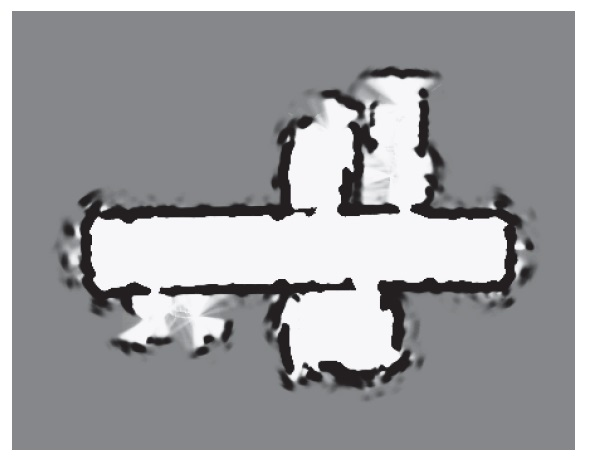
\includegraphics[width=0.7\linewidth]{95orig}}
	\caption{ ( Рис. 9.5 Карта вероятности занятости офисной среды, построенная на основе измерений сонара. Изображение принадлежат Кириллу Стачнису из Университета Фрайбурга (Cyrill Stachniss, University of Freiburg).)}
	\label{fig:95orig}
\end{figure}

\begin{figure}[H]
	\center{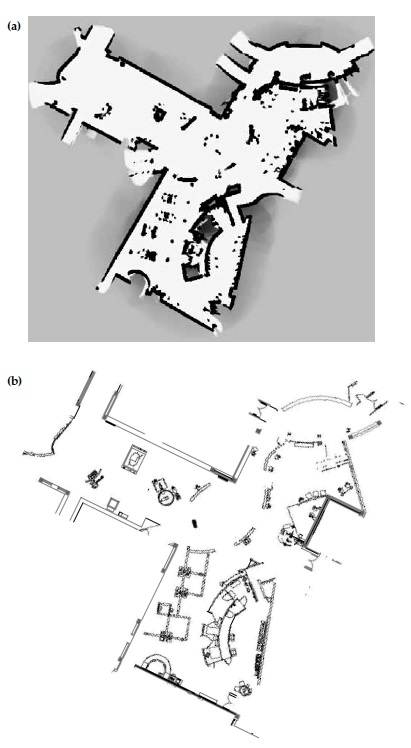
\includegraphics[width=0.9\linewidth]{96orig}}
	\caption{ ( Рис. 9.6 (a) Карта сетки занятости и (b) архитектурный план большого пространства выставки. Заметны мелкие неточности плана.)}
	\label{fig:96orig}
\end{figure}

\begin{figure}[H]
	\center{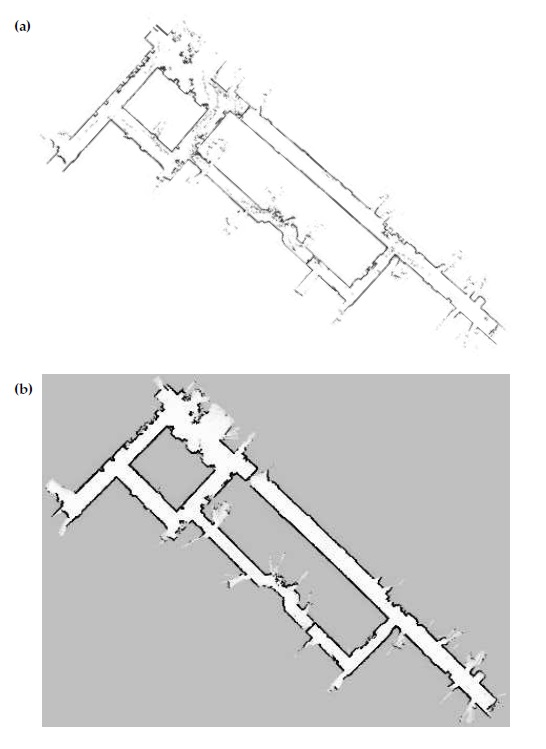
\includegraphics[width=0.9\linewidth]{97orig}}
	\caption{ ( Рис. 9.7 Исходные данные сканирования расстояний лазером  для скорректированного положения робота. Каждой точке соответствует обнаружение препятствия. Большинство препятствий статические (например, стены), но имеются и  динамические, поскольку во время сбора данных рядом с роботом ходят люди (a). Карта сетки занятости, построенная на этих данных. Интенсивность серого соответствует вероятности: чёрный соответствует высокой вероятности того, что ячейка занята, белый – высокой вероятности того, что она свободна. Серый фон отображает априорное распределение (b). Рис. (a) принадлежит Стефену Гатманну (Steffen Gutmann).)}
	\label{fig:97orig}
\end{figure}

\begin{figure}[H]
	\center{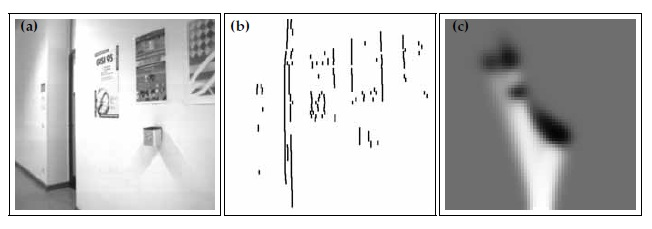
\includegraphics[width=1\linewidth]{98orig}}
	\caption{ ( Рис. 9.8 оценка карт сетки занятости на основе изображения со стереокамеры: изображение с камеры (a),  разреженная карта диспаратности (b), карта занятости после проекции изображения диспаратности на плоскость и свёртки результата гауссовой функцией (c). Изображения принадлежат Торстену Фролингаусу (Thorsten Fröhlinghaus))}
	\label{fig:98orig}
\end{figure}

На Рис. 9.7 сравниваются исходный набор данных и карта сетки занятости, сгенерированная на основе этих данных. Данные на панели (a) были предварительно обработаны алгоритмом SLAM таким образом, чтобы положения робота совпадали с картой. Часть данных повреждена из-за присутствия людей, но карта сетки занятости достаточно хорошо отфильтровывает людей. Это делает карты сетки занятости значительно более подходящими для навигации робота по сравнению со данными конечных точек сканирования, поскольку планировщик, принимающий на вход сырые данные конечных точек измерений, с большим трудом будет способен найти путь между близко расположенными препятствиями, даже если вероятность того, что ячейка свободна превышает вероятность того, что она занята. 

Заметим, что этот алгоритм принимает решения о занятости ячейки на основании данных измерений. Альтернативным источником информации является положение самого робота: при положении робота $x_t$, область вокруг $x_t$ должна быть свободной. Алгоритм обратного измерения в Таблице 9.2 можно легко модифицировать для учёта этой информации, путем возвращения большого отрицательного числа для всех ячеек сети, которые занимает робот, находясь в $x_t$. На практике следует учитывать размеры робота, особенно, если в процессе построения карты в среде присутствуют люди.\\ 

\textbf{9.2.1	Слияние данных нескольких типов датчиков}\\

Роботы часто оснащены более чем одним типом датчиков, поэтому естественным решением является интеграция информации на единой карте. Вопрос о наилучшем способе интеграции данных от нескольких датчиков особенно интересен, если датчики имеют разные характеристики. Например, на Рис. 9.8 показаны карты занятости, построены стереосистемой компьютерного зрения, в которой диспаратность проектируется на плоскость и сворачивается с помощью гауссовой функции. Конечно, характеристики стереоизображения отличны от данных расстояния ультразвукового датчика, поскольку разные датчики чувствительны для разных типов препятствий.

К сожалению, слияние данных от различных датчиков с помощью байесовских фильтров – задача крайне нетривиальная. Наивным решением будет запуск алгоритма \textbf{occupancy\_grid\_mapping} в Таблице 9.1 с разными модальностями датчиков. Такой подход имеет очевидный недостаток. Если разные датчики обнаруживают разные типы препятствий, результат байесовской фильтрации будет неточным. Допустим, препятствие может быть распознано одним типом датчика, но не обнаруживается другим. Тогда два разных типа датчиков будут генерировать противоречивую информацию, а результирующая карта – зависеть от количества подтверждающей информации, полученной от каждой системы. Обычно это нежелательно, поскольку занятость ячейки начнёт зависеть только от относительной частоты опроса датчиков.

Популярным методом интеграции информации от нескольких датчиков является построение раздельных карт для каждого типа датчика с последующей интеграцией карт подходящей комбинирующей функцией. Пусть $m^k = \{\textbf{m}_i^k\}$ определяет карту, построенную на основе $k$-го типа датчика. Если измерения датчиков независимы друг от друга, можно напрямую комбинировать их, используя \textit{законы де Моргана}\\

(9.9)
$$p(\textbf{m}_i)=1-\prod_k(1-p(\textbf{m}_i^k))$$

Возможно также вычислить максимум\\

(9.10)
$$p(\textbf{m}_i)=\underset{k}{\text{max}}\,\,p(\textbf{m}_i^k)$$

всех карт, отражающий наиболее пессимистичные оценки всех компонентов. Если хотя бы один из датчиков показывает, что ячейка занята, она будет занята на комбинированной карте.\\

\textbf{9.3	Обучающиеся обратные модели измерений}\\

\textbf{9.3.1	Инвертируем модель измерений}\\

Алгоритм картографирования на основе сетки занятости требует маргинализированной \textit{обратной модели измерений} $p(\textbf{m}_i | x, z)$. Эта вероятность называется «обратной» поскольку показывает зависимость событий от причин, давая информацию об изменении окружающего мира в результате измерения, в свою очередь, вызванном окружающей средой. Результатом является выражение для $i$-й ячейки сети, а полная инверсия будет давать вероятность $p(m | x, z)$. При изучении основного алгоритма в Таблице 9.2 была представлена специальная процедура для обратной модели. Возникает вопрос, возможно ли получить обратную модель в более точном виде, если имеется обычная модели измерения.

Это возможно, но несколько сложнее, чем кажется на первый взгляд. Теорема Байеса гласит\\

(9.11)
\begin{equation*}
\begin{split}
p(m|x,z)&=\frac{p(z|x,m)\,p(m|x)}{p(z|x)}\\
&=\eta\,p(z|x,m)\,p(m)
\end{split}
\end{equation*}

Здесь по умолчанию подразумевается $p(m | x) = p(m)$, поскольку положение робота ничего не говорит о карте (допущение, которое будет сделано в целях удобства). Если нашей целью было вычисление обратной модели для всей карты, этого допущения будет достаточно. Но алгоритм картографирования на основе сеток занятости аппроксимирует апостериорное разделение по картам через их маргиналы, по одному для каждой ячейки сетки $m_i$. Обратная модель для $i$-й ячейки сетки получается выбором маргинала соответствующей ячейки:\\

(9.12)
$$p(\textbf{m}_i|x,z)=\eta\sum_{m:m(i)=\textbf{m}_i}p(z|x,m)\,p(m)$$

В этом выражении суммируются все карты $m$ со значением занятости ячейки сетки $i$ равным $\textbf{m}_i$. Вообще-то, эту сумму нельзя вычислить, поскольку пространство всех карт слишком велико.\\

ОБУЧЕНИЕ С УЧИТЕЛЕМ\\

Опишем алгоритм аппроксимации этого выражения. Алгоритм включает генерацию значений из модели измерений, и аппроксимацию обратной модель с помощью \textit{алгоритма обучения с учителем}, например,  \textit{логистической регрессии} или \textit{искусственной нейронной сети}.\\

\textbf{9.3.2	Выборка элементов из прямой модели}\\

Основная идея проста и достаточна универсальна: если получится сгенерировать случайные триплеты из положений $x_t^{[k]}$, измерений $z_t^{[k]}$, и значений занятости карты $\textbf{m}_i^{[k]}$  для произвольной ячейки сети $\textbf{m}_i$, тогда получится обучить функцию, принимающую на вход положение $x$ и измерение $z$, и возвращающую вероятность занятости ячейки $\textbf{m}_i$.

Элемент вида $(x_t^{[k]}\,\,z_t^{[k]}\,\,\textbf{m}_i^{[k]})$ может быть сгенерирован следующей процедурой.\\

1.	Выбрать случайную карту $m^{[k]}\sim p(m)$. Например, можно извлечь случайную карту из имеющихся в наличии базы данных карт, которые представляют $p(m)$.\\

2. Выбрать положение $x_t^{[k]}$ внутри карты. Можно смело считать, что положения распределены равномерно.\\

3.	Выбрать измерение $z_t^{[k]}\sim p(z|x_t^{[k]},m^{[k]})$. Этот этап выборки напоминает симулятор робота, который случайным образом имитирует измерение датчика.\\

4.	Извлечь искомое «истинное» значение занятости $\textbf{m}_i$ для целевой ячейки сети карты $m$.\\

Результатом является выбранные положение $x_t^{[k]}$, измерение $z_t^{[k]}$, и значение занятости для ячейки сетки $\textbf{m}_i$. Повторное применение выборки даст набор данных

$$x_t^{[1]}\quad z_t^{[1]}\quad\longrightarrow\quad\text{occ}(\textbf{m}_i)^{[1]}$$
$$x_t^{[2]}\quad z_t^{[2]}\quad\longrightarrow\quad\text{occ}(\textbf{m}_i)^{[2]}$$
$$x_t^{[3]}\quad z_t^{[3]}\quad\longrightarrow\quad\text{occ}(\textbf{m}_i)^{[3]}$$
$\hspace{40mm}\vdots\hspace{8mm}\vdots\hspace{23mm}\vdots$

ОБУЧАЮЩИЕ ПРИМЕРЫ\\

Эти триплеты могут служить \textit{обучающими примерами}для алгоритма обучения с учителем, который аппроксимирует искомую условную вероятность $p(\textbf{m}_i|z,x)$. Здесь измерения $z$ и положение $x$ являются входными переменными, а значение занятости $\text{occ}(\textbf{m}_i)$ - целью для вывода алгоритма.

Такой подход неэффективен, поскольку не способен проявлять ряд следующих свойств, которые, как мы знаем, будут иметь место для обратной модели датчика.\\

•	Измерение не должно содержать информации о ячейках сетки вдали от расстояния восприятия. Это наблюдение влечёт два последствия. Во-первых, можно ограничить процессе генерирования элементов только триплетами, для которых ячейка $\textbf{m}_i$ находится внутри конуса измерений. Во-вторых, при формулировке гипотезы для ячейки необходимо включить только подмножество данных в измерение $z$ (то есть ближайшие бины) в качестве входа обучающегося алгоритма.\\

•	Характеристики датчика инвариантны по отношению к абсолютным координатам робота или ячейке сетки при выполнении измерения. Имеют значения только относительные координаты. Если обозначить положение робота через $x_t=(x\,\,y\,\,\theta)^T$, а координаты ячейки сети как $m_i=(x_{m_i}\,\,y_{m_i})^T$, то они будут проецироваться на локальную систему координат с помощью следующих операций переноса и поворота:\\

\begin{minipage}{0.2\textwidth}
\begin{equation*}
\left(\begin{array}{cc}
\cos\theta&-\sin\theta\\
\sin\theta&\cos\theta\\
\end{array}\right)
\left(\begin{array}{c}
x_{\textbf{m}_i}\,-x\\
y_{\textbf{m}_i}\,-y\\
\end{array}\right)
\end{equation*}
\end{minipage}\\

В роботах с круговыми массивами датчиков расстояния имеет смысл кодировать относительное местонахождение ячейки сети, используя уже знакомые полярные координаты (расстояние и угол направления).\\

•	Близлежащие ячейки сетки должны иметь схожую интерпретацию для обратной модели датчика. Это свойство гладкость подразумевает, что может оказаться выгодным обучить простую функцию с координатами ячейки сети в качестве входных данных, чем обучать отдельную функцию для каждой ячейки сети.\\

•	Если у робота имеются функционально идентичные датчики, обратная модель датчика должна быть взаимозаменяемой для различных моделей датчиков. Для роботов, оборудованных круговым массивом датчиков расстояния, любой из результирующих лучей датчика характеризуется одной и той же обратной моделью датчика.\\

Самый простой способ обеспечить такую инвариантность - это ограничить обучающийся алгоритм выбором соответствующих входных переменных. Хорошим решением будет использование информации о положении, таким образом, чтобы обучающийся алгоритм не мог формулировать решение на основе абсолютных координат. Также стоит отбросить измерения датчика, для которых известно, что они иррелеванты по отношению к прогнозам занятости и ограничить прогноз только ячейками внутри поля измерения датчика. Используя это постоянство, размер тренировочного набора можно существенно уменьшить.\\

\textbf{9.3.3	Функция ошибок}\\

Для тренировки обучающегося алгоритма понадобится оценочная функция ошибки. Популярным примером являются искусственные нейронные сети, тренированные с алгоритмом обратного распространения.\\
ОБРАТНОЕ РАСПРОСТРАНЕНИЕ\\
Обратное распространение обучает \textit{нейронные сети} с помощью \textit{градиентного спуска} в пространстве параметров. Заданная функция ошибки, измеряющая «разницу» между текущим и искомым выводом, обратное распространение вычисляет первую производную целевой функции и параметров нейронной сети, и настраивает параметры в направлении, обратном градиенту, чтобы уменьшить разницу. Поэтому возникает вопрос о том, какую функцию ошибки использовать.

Общепринято обучать алгоритм таким образом, чтобы максимизировать логарифм правдоподобия обучающих данных. Пусть дан обучающий набор данных следующего вида\\

(9.13)
$$\text{input}^{[1]}\quad\longrightarrow\quad\text{occ}(\textbf{m}_i)^{[1]}$$
$$\text{input}^{[2]}\quad\longrightarrow\quad\text{occ}(\textbf{m}_i)^{[2]}$$
$$\text{input}^{[3]}\quad\longrightarrow\quad\text{occ}(\textbf{m}_i)^{[3]}$$
$\hspace{45mm}\vdots\hspace{25mm}\vdots$

$\text{occ}(\textbf{m}_i)^{[k]}$ - это $k$-й элемент искомой условной вероятности, а $\text{input}^{[k]}$ - соответствующий вход обучающегося алгоритма. Точная форма входных данных может отличаться как результат кодирования известной инвариантности, но точный вид входной функции не играет никакой роли в форме функции ошибки.

Давайте определим параметры обучающегося алгоритма через $W$. Допустим, что каждый отдельный элемент в обучающих данных был сгенерирован независимо, тогда правдоподобие обучающих данных будет равно\\

(9.14)
$$\prod_i p(\textbf{m}_i^{[k]}|\text{input}^{[k]},W)$$

а дополнение логарифма\\

(9.15)
$$J(W)=\,-\sum_i \log p(\textbf{m}_i^{[k]}|\text{input}^{[k]},W)$$

Здесь $J$ определяет функцию, которую необходимо минимизировать в процессе обучения.

Давайте определим обучающийся алгоритм $f (\text{input}^{[k]},W)$. Выход функции – это значение в интервале $\left[ 0;1\right] $. После обучения обучающийся алгоритм должен выдавать значения занятости:\\

(9.16)
\begin{equation*}
p(\textbf{m}_i^{[k]}|\text{input}^{[k]},W) = \left\{
\begin{array}{ll}
f(\text{input}^{[k]},W)& \mbox{если}\,\,\textbf{m}_i^{[k]}=1 \\
1-f(\text{input}^{[k]},W)& \mbox{если}\,\,\textbf{m}_i^{[k]}=0
\end{array}
\right.
\end{equation*}

Таким образом, выполняется поиск функции ошибки для подстройки $W$ так, чтобы минимизировать отклонение прогнозируемой вероятности от 
одного из примеров обучения. Чтобы найти такую функцию ошибки, перепишем (9.16) в следующем виде:\\

(9.17)
$$p(\textbf{m}_i^{[k]}|\text{input}^{[k]},W) = f(\text{input}^{[k]},W)^{\textbf{m}_i^{[k]}}(1-f(\text{input}^{[k]},W))^{1-\textbf{m}_i^{[k]}}$$

Легко заметить, что это произведение и выражение (9.16) идентичны. В произведении один из членов всегда равен 1, поскольку экспонента равна нулю. Подстановка произведения в (9.15) и умножение результата на минус один даёт следующую функцию:\\

(9.18)
\begin{equation*}
\begin{split}
J(W)&=\,-\sum_i\log\left[f(\text{input}^{[k]},W)^{\textbf{m}_i^{[k]}}(1-f(\text{input}^{[k]},W))^{1-\textbf{m}_i^{[k]}}\right]  \\
&=\,-\sum_i \textbf{m}_i^{[k]}\log f(\text{input}^{[k]},W)+(1-\textbf{m}_i^{[k]})\log (1-f(\text{input}^{[k]},W))
\end{split}
\end{equation*}

$J(W)$ – это функция ошибки, которую требуется минимизировать при обучении алгоритма. Она легко укладывается в любой алгоритм, который использует градиентный спуск для настройки параметров.\\

\textbf{9.3.4	Примеры и дальнейшие соображения}\\

На Рис. 9.9 показан результат искусственной нейронной сети, обученной имитировать обратную модель датчика. В этом примере робот оборудован круговым массивом ультразвуковых датчиков, установленном, приблизительно, на уровне высоты стола. На вход сети подаются относительное расстояние и направление на целевую ячейку, а также набор из пяти связанных измерений расстояния. На выходе будет вероятность занятости: чем темнее ячейка, тем вероятнее она занята. Как показывает пример, метод верно обучается различать свободное и занятое пространство. Равномерная серая окраска за препятствиями соответствует априорной вероятности занятости, поэтому в алгоритме картографирования с помощью сеток занятости ничего не изменяется. На Рис. 9.9b показаны ошибочно короткие показания датчика слева снизу. Здесь одиночного сканирования недостаточно для прогнозирования препятствия с высокой вероятностью.

\begin{figure}[H]
	\center{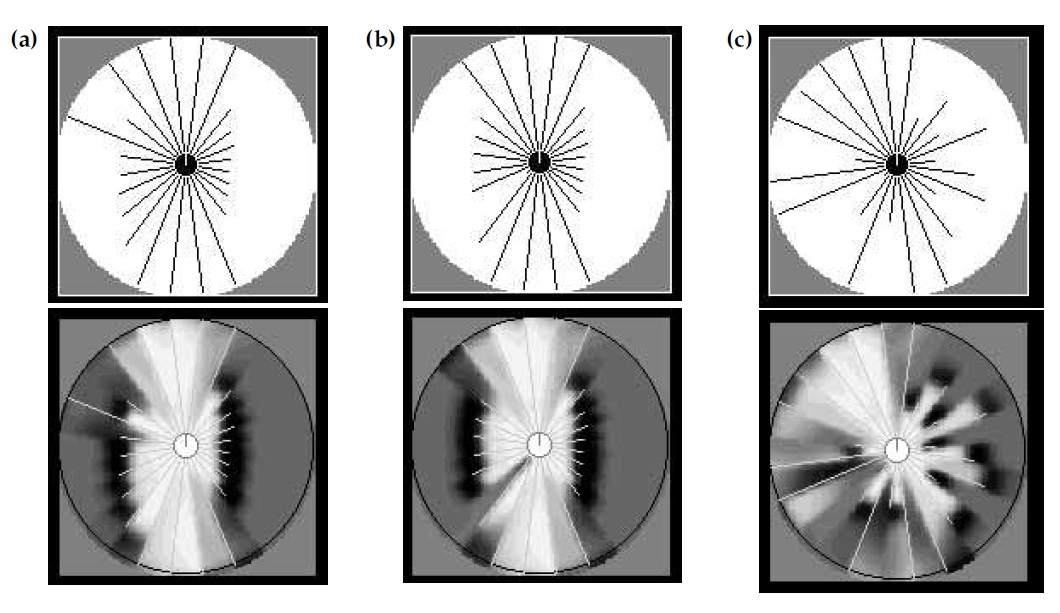
\includegraphics[width=0.9\linewidth]{99orig}}
	\caption{ ( Рис. 9.9 Обратная модель датчика, обученная на данных: три значения сканирования сонара (верхний ряд) и локальные карты занятости (нижний ряд), сгенерированные нейронной сетью. Яркие области означают свободное пространство, а тёмные означают проходы сканирования и препятствия (увеличенные на диаметр робота).)}
	\label{fig:99orig}
\end{figure}

Заметим, что существует множество способов обучить оценивающую функцию на основе данных, собранных роботом, вместо имитационных данных из прямой модели. В общем, это самые точные данные, которые возможно использовать для обучения, поскольку модель измерения всегда является лишь приближением. Одним из таких способов является робот, действующий в известной среде с известной картой. Используя марковскую локализацию, возможно выполнить локализацию, а затем использовать текущие измерения и известную карту занятости в качестве тренировочных примеров.  Сначала возможно использовать даже приблизительную карту и обученную модель датчика для того, чтобы сгенерировать лучшую карту, и использовать только что описанную процедуру для улучшения обратной модели измерений.\\

\textbf{9.4	Картографирование на основе максимумов апостериорной занятости }\\

\textbf{9.4.1	Необходимость сохранения зависимостей}\\

В оставшейся части главы вернёмся в одному из самых базовых допущений алгоритма картографирования с помощью сеток занятости. В разделе 9.2 было сделано допущение о том, что можно безопасно  разложить задачу получения карты, определённую в пространстве высокой размерности для всех карт, на совокупность задач картографирования единичных ячеек. Это допущение привело к следующей факторизации (9.4):\\

(9.19)
$$p(m|z_{1:t},x_{1:t})=\prod_i p(\textbf{m}_i|z_{1:t},x_{1:t})$$

Возникает вопрос, насколько следует доверять результату любого алгоритма на основе полной декомпозиции.

\begin{figure}[H]
	\center{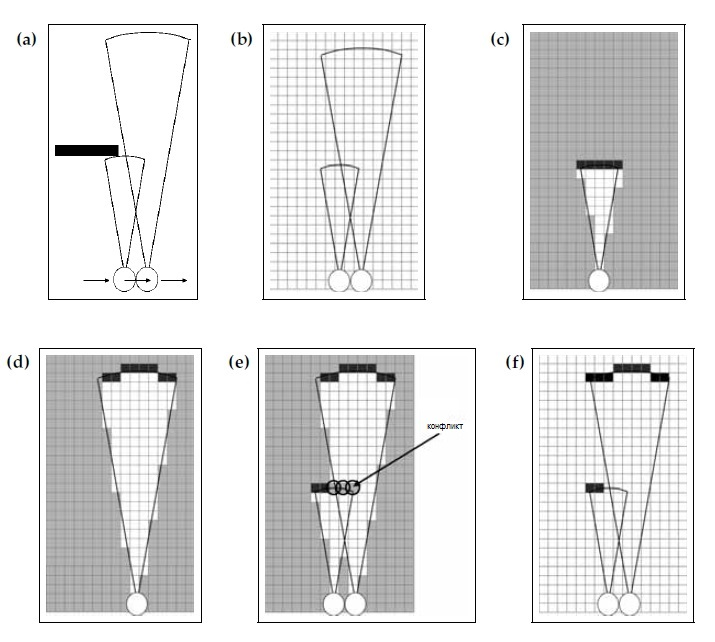
\includegraphics[width=0.9\linewidth]{910orig}}
	\caption{ ( Рис. 9.10 Проблема стандартного алгоритма картографирования с использованием сеток занятости из раздела 9.2. Для среды, показанной на Рисунке (a), проходящий робот может получить (идеальное) измерение, показанное на схеме (b). Метод факторизации по отдельности проецирует эти лучи для каждой ячейки сети и каждого луча, как показано на схемах (c) и (d). Результатом комбинирования обоих интерпретаций становится карта, показанная на схеме (e). Очевидно, имеются конфликтующие пересечения, показанные на схеме (e) в виде кругов. Интересным наблюдением является то, что существуют карты, показанные на схеме (f), объясняющие измерения карт безо всяких конфликтов. Для показаний датчиков, которые требуются объяснить, достаточно допустить, что препятствие находится где-то в конусе измерений, а не повсеместно.)}
	\label{fig:910orig}
\end{figure}

На Рис. 9.10 показана задача, являющаяся прямым результатом такой факторизации. В данном случае робот, обращённый в сторону стены, принимает два идеальных измерения расстояния сонаром. Поскольку подход на основе множителей прогнозирует объект по всей дуге измеренного расстояния, значения занятости по всем ячейкам сетки вдоль дуги возрастают. При комбинировании двух разных измерений, показанных на Рис. 9.10c и d, получается конфликт, показанный на Рис. 9.10e. Стандартный алгоритм картографирования на основе сеток занятости «разрешает» этот конфликт суммированием положительных и отрицательных свидетельств занятости ячеек, но результат будет отражать отрицательные частоты двух типов измерений, что нежелательно. 

Однако, существуют карты, наподобие показанное на Рис. 9.10f, которые объясняют измерения датчика безо всяких конфликтов. Это происходит потому, что для показаний датчика, которые необходимо объяснить достаточно допустить, что препятствие находится где-то в конусе измерения. Другими словами, факт того, что конус измерения проходит через несколько ячеек, выявляет важные зависимости между соседними ячейками сети. При декомпозиции картографирования для тысяч задач оценки ячейки сети возможность учёта этих зависимостей будет утеряна. 

\begin{table}[H]
\begin{center}
\begin{tabular}{|l|}
\hline
{}\\
1: \textbf{Algorithm MAP\_occupancy\_grid\_mapping}$(x_{1:t},z_{1:t}):$ \\
2:\hspace{5mm}$\textit{установить}\,\,m=\{0\}$\\
3:\hspace{5mm}$\textit{повторять до сходимости}$\\
4:\hspace{10mm}$\textit{Для всех ячеек}\,\,\textbf{m}_i\,\,\textit{do}$\\
5:\hspace{15mm}$m_i=\underset{k=0,1}{\text{argmax}}\,\,k\,\,l_0+\sum_t \log$\\
\hspace{25mm}$\textbf{measurement\_model} (z_t,x_t,m\,\textit{для}\,\,\textbf{m}_i=k)$\\
6:\hspace{10mm}$\textit{endfor}$\\
7:\hspace{5mm}$\textit{endrepeat}$\\
8:\hspace{5mm}$\textit{return}\,\,m$\\
{}\\
\hline
\end{tabular}
\caption{(Таблица 9.3 Алгоритм максимума апостериорной занятости сетки, использующий стандартные модели измерения вместо обратных моделей.)}
\end{center}
\end{table}

\textbf{9.4.2	Картографирование с помощью сеток занятости, используя прямые модели}\\

Эти зависимости учитываются алгоритмом, который выводит моду апостериорного распределения, вместо полного распределения. Мода определяется как максимум логарифма апостериорной вероятности карты:\\

(9.20)
$$m^*=\underset{m}{\text{argmax}}\log p(m|z_{1:t},x_{1:t})$$

Апостериорная вероятность карты умножается на априорную и правдоподобие измерения (см. Выражение (9.11)):\\

(9.21)
$$\log p(m|z_{1:t},x_{1:t})=\text{const.}+\log p(z_{1:t}|x_{1:t},m)+\log p(m)$$

Логарифм правдоподобия $\log p(z_{1:t}|x_{1:t},m)$ разбивается на сумму логарифмов правдоподобия отдельных измерений:\\

(9.22)
$$\log p(z_{1:t}|x_{1:t},m)=\sum\log p(z_t|x_t,m)$$

Более того, логарифм априорной вероятности тоже можно подвергнуть декомпозиции. Заметим, что априорная вероятность любой карты $m$ задана следующим произведением:\\

(9.23)
\begin{equation*}
\begin{split}
p(m)&=\prod_i p(\textbf{m})^{\textbf{m}_i}(1-p(\textbf{m}))^{1-\textbf{m}_i} \\
&=(1-p(\textbf{m}))^N\prod_i p(\textbf{m})^{\textbf{m}_i}(1-p(\textbf{m}))^{-\textbf{m}_i}\\
&=\eta\,\prod_i p(\textbf{m})^{\textbf{m}_i}(1-p(\textbf{m}))^{-\textbf{m}_i}
\end{split}
\end{equation*}

Здесь $p(\textbf{m})$ - априорная вероятность занятости (то есть, $p(\textbf{m}) = 0.5$), а $N$ - количество ячеек сетки на карте. Выражение $(1-p(\textbf{m}))^N$ является просто константой, которая заменяется общим символом $\eta$.

Теперь можно получить логарифмическую версию априорной вероятности:\\

(9.24)
\begin{equation*}
\begin{split}
\log p(m)&=\text{const.}+\sum_i \textbf{m}_i\log p(\textbf{m})-\textbf{m}_i\,\log(1-p(\textbf{m}))\\
&=\text{const.}+\sum_i \textbf{m}_i\log\frac{p(\textbf{m})}{1-p(\textbf{m})}\\
&=\text{const.}+\sum_i \textbf{m}_i\,l_0
\end{split}
\end{equation*}

Константа $l_0$ берётся из (9.7). Член $M log(1-p(\textbf{m}_i))$ очевидно, не зависит от карты. Поэтому, достаточно оптимизировать правдоподобие оставшегося выражения и данных:\\

(9.25)
$$m^*=\underset{m}{argmax}\sum_t \log p(z_t|x_t,m)+l_0\sum_i \textbf{m}_i$$

Алгоритм поиска экстремума для логарифма вероятности приводится в Таблице 9.3. Он начинается с полностью пустой карты (строка 2). Он «переворачивает» значение занятости ячейки сети, когда правдоподобие переворота превышает правдоподобие данных (строки 4-6).  Для этого алгоритма важно, чтобы априорная вероятность занятости $p(\textbf{m}_i)$ не была слишком близка к 1, в противном случае, результатом будет карта со всеми занятыми ячейками. Для любого алгоритма поиска экстремума этот метод гарантирует только нахождение локального максимума. На практике локальных максимумов обычно немного, если они вообще есть.

\begin{figure}[H]
	\center{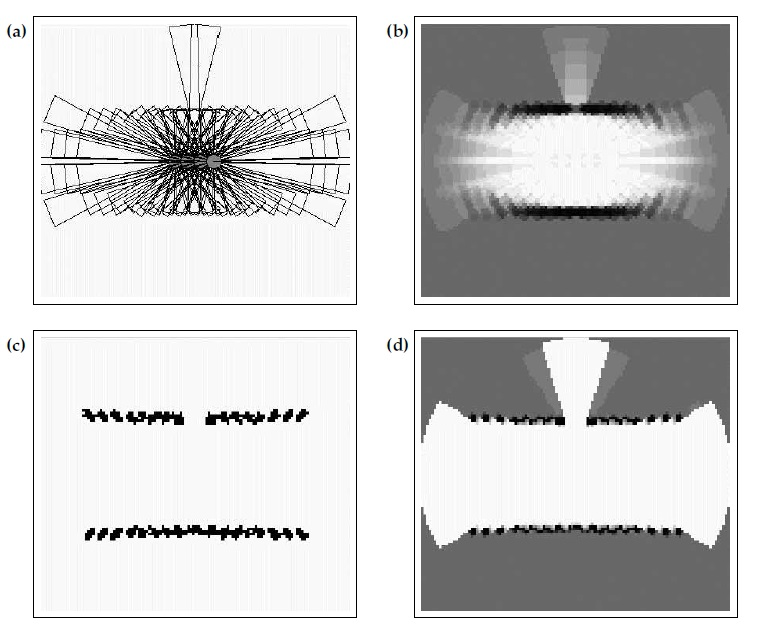
\includegraphics[width=0.9\linewidth]{911orig}}
	\caption{ ( Рис. 9.11 Измерения дальности сонаром из идеальной имитации (a). Результаты стандартного алгоритма классификации на основе занятости, за исключением открытой двери (b).  Максимум апостериорной карты (c). Остаточная неопределённость на карте, полученная измерениями чувствительности функции правдоподобия карты по отношению к отдельным ячейкам сетки (d). На этой карте чётко видна дверь, а также более ровные стены с обеих сторон.)}
	\label{fig:911orig}
\end{figure}

На Рис. 9.11 показан эффект алгоритма сетки занятости MAP. На Рис. 9.11a показан набор идеальных данных для робота, проходящего через открытую дверь. Некоторые из измерений сонара обнаруживают открытую дверь, но остальные отражаются от дверного косяка. Стандартный алгоритм картографирования на основе занятости с обратными моделями измерений неспособен обнаружить открытую дверь, как показано на Рис. 9.11b. Мода апостериорного распределения показана на Рис. 9.11c. Эта карта верно моделирует открытую дверь, поэтому она лучше подходит для навигации робота по сравнению со стандартным алгоритмом карты сетки занятости. На. Рис. 9.11d показана остаточная неопределённость карты. Эта схема является результатом анализа чувствительности по каждой ячейке: величина, на которую инверсия состояния ячейки уменьшает функцию логарифма правдоподобия показана насыщенностью серого цвета. Эта схема, похожая на обычную карту сетки занятости, показывает максимум неопределённости для ячеек сети, расположенных за препятствиями.

Существуют определённые ограничения алгоритма \textbf{MAP\_occupancy \_grid\_mapping}, и он может быть улучшен различными способами. Алгоритм максимизирует апостериорную вероятность и не возвращает никаких данных о неопределённости карты. Анализ чувствительности аппроксимирует эту неопределённость, но с чрезмерно оптимистической оценкой, поскольку проверяется только локальная мода. Более того, алгоритм является пакетным и не может выполняться последовательно. Фактически, алгоритм MAP требует хранения всех данных в памяти. С вычислительной стороны, алгоритм можно ускорить инициализацией результатом работы обычного метода картографирования с помощью сетки занятости вместо пустой карты. Наконец, заметим, что только небольшое число измерений подвержены перевороту ячейки сети в строке 5 Таблицы 9.3. Хотя каждая сумма потенциально велика, при вычислении argmax необходимо проверить только небольшое количество элементов. Это свойство можно использовать в базовом алгоритме для увеличения вычислительной эффективности.\\

\textbf{9.4	Выводы}\\

В этой главе представлены алгоритмы обучающихся сеток занятости. Во всех представленных алгоритмах требуется точная оценка положения робота, поскольку они не решают проблему глобального построения карт.\\

•	Стандартный алгоритм картографирования на основе определения занятости каждой отдельной ячейки оценивает апостериорную вероятность занятости и представляет собой адаптацию бинарного байесовского фильтра для статических сред.\\

•	Данные с нескольких датчиков могут быть объединены на одной карте двумя способами: поддержания единственной карты с помощью байесовских фильтров и поддержанием нескольких карт, по одной для каждого типа датчика. Предпочтителен обычно второй подход, поскольку разные датчики чувствительны к разным типам препятствий.\\

•	Стандартный алгоритм картографирования на основе занятости основан на обратных моделях измерения, идущих от следствия (измерения) к причинам (занятости). Это отличается от предыдущих реализаций байесовских фильтров в контексте локализации, поскольку они были основаны на обычной модели измерения, связывающей причину со следствием.\\

•	Возможно обучить обратные модели датчиков на основе обычной модели измерений, моделирующей датчик от причины к следствию. Чтобы это сделать, необходимо сгенерировать выборку и обучить обратную модель, используя алгоритм обучения с учителем.\\

•	Стандартный алгоритм картографирования на основе занятости не поддерживает зависимости оценок занятости. Это является результатом декомпозиции задачи апостериорной оценки карты на большое число задач апостериорной оценки единичных ячеек.\\

•	Апостериорное значение для всей карты обычно не вычислимо из-за большого количества карт, которые можно определить на сетке. Однако, его возможно максимизировать, что позволит создавать карты, в большей степени соответствующие данным по сравнению с алгоритмами сетки занятости на основе байесовских фильтров. Но для выполнения максимизации требуется доступность всех данных, а результирующий максимум апостериорной карты не сохраняет остаточную неопределённость карты.\\

Без сомнения, карты сетки занятости и их различные варианты чрезвычайно популярны в робототехнике в силу их простоты получения и сохранения важных для навигации робота элементов. \\

\textbf{9.6	Библиографические примечания}\\

Карты сеток занятости были введены Элфисом (Elfes, 1987), в кандидатской диссертации которого (1989) была определена предметная область. Известная статья Моравица (Moravec, 1988) дала очень доступную формулировку задачи, заложив базовый вероятностный метод, который составляет суть этой главы. В неопубликованной работе Моравица и Мартина (Moravec and Martin,1994) карты сетки занятости были обобщены до 3-D со стереокамерой в качестве основного датчика. Слияние данных нескольких датчиков в сетках занятости было впервые описано в работе Труна (Thrun et al., 1998a). Результат обучения обратных моделей датчиков, описанных в этой главе, можно найти в работе Труна (Thrun, 1998b). Метод прямого моделирования, также описанный в этой главе, основан на похожем алгоритме Труна (Thrun,  2003).

Карты занятости были использованы в целом ряде различных областей. Боренштейн и Корин (Borenstein and Koren, 1991) первыми применили карты сетки занятости к задаче предотвращения столкновений. Многие авторы использовали карты сетки занятости для задачи локализации перекрёстным сравнением двух карт. Такие алгоритмы «наложения карт» детально обсуждались в Главе 7. Бисвас (Biswas et al., 2002) использовал карты сеток занятости для обучения модели определения формы подвижных объектов в динамических средах. Этот метод позже был расширен до обучения иерархических классов моделей динамических объектов, представленных в виде карт сетки занятости (Anguelov et al. 2002). Карты сетки занятости также активно использовались в контексте одновременной локализации и картографирования. Эти области применения будут обсуждаться ниже.

Идея представления пространства является только одной из многих идей, исследуемых в литературе по мобильной робототехнике. Классические работы по планированию движения часто полагаются на представление среды в виде полигонов, но не раскрывают, каким образом эти модели были получены из данных (Schwartz et al. 1987). Ранние работы по построению полигональных карт были выполнены Чатила и Лаумондом (Chatila and Laumond, 1985). Первая реализация, использующая калмановские фильтры для соединения прямых, полученных из данных сонара, была выполнена Краули (Crowley, 1989). В более новой работе Ангелов (Anguelov et al., 2004) предложил методы идентификации прямых линий дверей из сырых данных датчиков, а также изучил визуальные атрибуты для улучшения коэффициента обнаружения двери.

\begin{figure}[H]
	\center{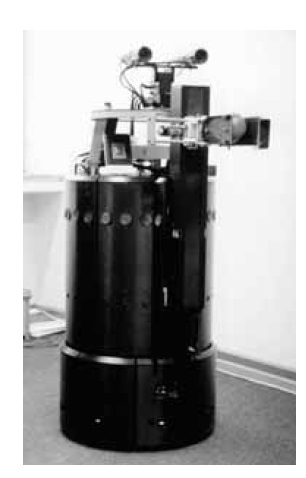
\includegraphics[width=0.4\linewidth]{912orig}}
	\caption{ ( Рис. 9.12 Мобильный робот для работы в помещениях типа RWI B21, оснащённый 24 ультразвуковыми датчиками, смонтированными в круговой массив вокруг робота.)}
	\label{fig:912orig}
\end{figure}

ПРОСТРАНСТВЕННАЯ СЕМАНТИЧЕСКАЯ
ИЕРАРХИЯ\\
Ранние идеи пространственного отображения топологической парадигмы, в которой пространство представлено в виде набора локальных областей, часто соответствует отдельным действиям робота по навигации между соседними местоположениями. Примеры топологического картографирования включают работу Куперса и Левитта (Kuipers and Levitt, 1988) по \textit{пространственной семантической иерархии }(см также Kuipers et al., 2004)), магистерскую работу Матарика  (Mataric, 1990), работу Кортенкампа и Веймауса (Kortenkamp and Weymouth, 1994) по топологическим графам, полученным из визуальных данных и данных ультразвуковых датчиков, и метод Шатки и Кэлблинга (Shatkay and Kaelbling, 1997) по использованию пространственных HMM с информацией о длине дуги. Карты сетки занятости используют родственную прадигму метрического отображения. Метрическое выражение прямо описывает среду робота в некоторой абсолютной координатной системе. Вторым примером метрического подхода является алгоритм EKF SLAM который будет обсуждаться в следующей главе.

Было сделано множество попыток создать алгоритмы картографирования, сочетающие лучшее обеих парадигм, топологической и метрической. Томатис (Tomatis et al., 2002) применил топологические выражения к непротиворечивому замыканию циклов, переводя их затем в метрические карты. Трун (Thrun, 1998b) первым построил метрическую карту сетки занятости, а затем предложил топологическую основу для быстрого планирования движения. В Главе 11 будут изучены методы, соединяющие обе парадигмы, метрическую и топологическую.\\

\textbf{9.7	Упражнения}\\

1.	Изменить базовый алгоритм сетки занятости в Таблице 9.1, включив учёт изменения занятости со временем. Для учёта таких изменений, доказательства, собранные $\varDelta t$ тактов времени назад, должны быть уменьшены в $\alpha^{\varDelta t}$ раз для некоего значения $\alpha<1(\text{например}, \alpha=0,99)$.\\
ЭКСПОНЕНЦИАЛЬНОЕ ЗАТУХАНИЕ \\
Такое правило называется \textit{экспоненциальным затуханием.} Привести алгоритм построения карт с помощью сетки занятости и экспоненциального затухания в виде логарифма шансов и объяснить его правильность. Если не сможете найти точный алгоритм, привести приблизительный и объяснить, почему применимо предлагаемое приближение. Для простоты можно допустить априорную вероятность занятости $p(\textbf{m}_i) = 0.5$.\\

2.	Бинарный байесовский фильтр основан на допущениях, что ячейка может быть только занятой или свободной, а датчик даёт зашумлённые свидетельства в пользу верной гипотезы. В этом упражнении требуется построить альтернативный метод оценки ячейки сети: Допустим, датчик способен измерять только “0 = незанято” или “1 = занято”, и генерирует последовательность\\

0, 0, 1, 0, 1, 1, 1, 0, 1, 0.\\

Какого максимальное правдоподобие вероятности $p$ того, что следующее значение показания датчика будет 1? Привести инкрементную формулу общей оценивающей функции максимального правдоподобия для этой вероятности $p$. Обсудить разницу этой оценивающей функции и бинарного фильтра Байеса (только для отдельной ячейки).\\

3.	Мы уже изучили общую конфигурацию датчиков роботов для работы внутри помещений. Допустим, робот, находящийся в помещении, использует ультразвуковой датчик с углом раскрытия 15 градусов, установленный на фиксированной высоте горизонтально и параллельно полу. Такой робот показан на Рис. 9.12. Обсудить, что может произойти, если робот встретит препятствие, которое находится чуть ниже датчика (например, на 15 см ниже). В частности, ответить на следующие вопросы.\\

(a)	При каких условиях робот обнаружит препятствие? Когда не сможет обнаружить его? Привести краткий ответ.\\

(b)	Какие следствия это имеет для бинарного байесовского фильтра и лежащего в его основе марковского свойства? Как можно вывести из строя алгоритм занятости сетки?\\

(c)	На основе ответа на предыдущий вопрос можно ли предложить улучшенный алгоритм картографирования с помощью сетки занятости, который будет более надёжно обнаруживать препятствия по сравнению с базовым?\\

4.	В этом упражнении требуется разработать простую модель датчика. Допустим, даны бинарные измерения занятости для следующих четырёх ячеек:\\

\begin{table}[H]
\begin{center}
\begin{tabular}{|c|c|c|}
\hline
\text{Номер ячейки}&\text{Тип}&\text{последовательность}\\
\hline
\text{ячейка 1}&\text{занята}&1\quad1\quad0\quad1\quad0\quad1\quad1\\
\text{ячейка 2}&\text{занята}&0\quad1\quad1\quad1\quad0\quad0\quad1\\
\text{ячейка 3}&\text{свободна}&0\quad0\quad0\quad0\quad0\quad0\quad0\\
\text{ячейка 4}&\text{свободна}&1\quad0\quad0\quad1\quad0\quad0\quad0\\
\hline
\end{tabular}
\end{center}
\end{table}

Какова модель максимального правдоподобия измерения $p(z | \textbf{m}_i)$? (Подсказка: $\textbf{m}_i$ – бинарная переменная занятости, а $z$ – бинарная переменная измерения.)\\

5.	Для Таблицы из Упражнения 4 реализовать базовый алгоритм сетки занятости.\\

(a)	Какова апостериорная вероятность $p(\textbf{m}_i | z_{1:7})$ для четырёх разных случаев, если априорная $p(\textbf{m}_i) = 0,5$?\\

(b)	Привести алгоритм настройки для модели датчика приближающий вывод алгоритма картографирования на основе сетки занятости как можно ближе к истинным значениям для четырёх случаев в Упражнении 4. Что удалось найти? (В этом упражнении потребуется найти подходящую меру близости.)\\

6.	Стандартный алгоритм построения карт на основе сетки занятости реализован в виде логарифма шансов, хотя он также может быть реализован, используя вероятности.\\

(a)	Вывести обновлённое правило, напрямую выражающее вероятности занятости, без использования представления в виде логарифма шансов.\\

(b)	Для реализации на популярном языке программирования, например, C++, привести пример, в котором реализация вероятности даёт \textit{разные} результаты с реализацией в виде логарифма шансов, в силу разного числового представления. Объяснить ответ и обсудить, станет ли эта разница проблемой при практическом использовании.\\






 
\end{document}